% ----------------------------------------------------------
\chapter{Arquitetura}
% ----------------------------------------------------------

Após estudar os desdobramentos dos efeitos de órbita baixa e entender o que é necessário para se realizar um projeto confiável de computador de bordo de um nanossatélite, foi necessária a compreensão dos pré-requisitos de projeto. Com isso, foram escolhidos os componentes principais da placa, propondo-se uma arquitetura para o sistema, propondo um hardware confiável, robusto e versátil.  

\section{Pré-Requisitos de Projeto}

Como dito, foi preciso entender os pré-requisitos impostos para o OBDH da terceira geração do SpaceLab. Abaixo, na Tabela \ref{tab:Tab_Req}, se encontram os requisitos gerais do projeto, em conjunto com o pretexto e com o nível de prioridade.

\begin{longtable}{@{}p{5cm}p{5cm}p{3.5cm}@{}}
    \centering
	\ABNTEXfontereduzida
	\label{tab:Tab_Req}\tabularnewline
	\caption{Requisitos do projeto.}\tabularnewline
	%\begin{tabular}{@{}p{2cm}p{2cm}p{2cm}p{2cm}p{2cm}p{2cm}p{3cm}@{}}
	\hline
	\textbf{\centering{Descrição}} & \textbf{\centering{Pretexto}} & \textbf{\centering{Prioridade}} \tabularnewline
        \hline
        O módulo OBDH deve ser compatível com o padrão CubeSat & Assegura compatibilidade com outros satélites desenvolvidos no SpaceLab & Alta \tabularnewline
        
       \hline
        O módulo OBDH deve operar corretamente entre -40°C e 85°C & Para operar com segurança em um ambiente LEO & Alta \tabularnewline

       \hline
        O módulo OBDH deve possuir um microcontrolador capaz de usar um sistema Linux & Para gerenciar e coordenar operações dentro e fora do módulo, sendo capaz de realizar tarefas complexas  & Alta \tabularnewline

       \hline
        O módulo OBDH deve possuir uma memória DDR com capacidade de 512Mb (preferencialmente com ECC)  & Memória suficiente para operações do OBDH e armazenamento de dados  & Alta\tabularnewline

        \hline
        O módulo OBDH deve possuir uma memória FRAM para armazenar parâmetros de configuração & Provê memória não-volátil e duradoura, menos sucetível à radiação & Alta \tabularnewline 

        \hline
        O módulo OBDH deve possuir uma memória Flash para armazenar pacotes (preferencialmente com ECC) & Para armazenar dados e pacotes recebidos & Alta\tabularnewline 

        \hline
        O módulo OBDH deve possuir um WDT (\textit{Watchdog Timer}) para reiniciar o microcontrolador em caso de falha de \textit{software} & Reinicia automaticamente o microcontrolador caso haja a falha  & Alta \tabularnewline

        \hline
        O módulo OBDH deve possuir sensores de medição de tensão e corrente em suas tensões & Para monitoramento de potência consumida & Alta\tabularnewline

        \hline
        O módulo OBDH deve possuir proteção de sobrecorrente (20\% acima do valor nominal) & Para proteção contra \textit{latch-up}  & Alta \tabularnewline

        \hline
        O módulo OBDH deve possuir um giroscópio para medição de velocidade angular & Para permitir controle ativo do satélite  & Alta \tabularnewline 

       \hline
        O módulo OBDH deve possuir um magnetômetro & Para permitir controle ativo do satélite  & Alta \tabularnewline

        \hline
        O módulo OBDH deve possuir uma interface RS-422 para transmissão de mensagens de \textit{debug/log} e receber parâmetros de configuração & Comunicação de longa distância com maior imunidade ao ruído e maior taxa de dados (comparando com UART)  & Alta \tabularnewline

       \hline
        O módulo OBDH deve possuir uma interface CAN para receber e transmitir comandos e dados & Comunicação robusta e com suporte a múltiplos sistemas do CubeSat  & Alta\tabularnewline

        \hline
        O módulo OBDH deve possuir uma interface acessível externamente para programação do microcontrolador & Para o módulo ser facilmente programado pelo time  & Alta \tabularnewline

        \hline
        O módulo OBDH deve possuir uma interface para uma \textit{daughter board} & Para prover suporte a outras interfaces e periféricos  & Baixa \tabularnewline

        \hline
        O módulo OBDH deve possuir um sensor de temperatura com precisão menor ou igual a 1°C & Para prevenir danos de temperaturas extremas & Baixa\tabularnewline

        \hline
        O módulo OBDH deve possuir uma interface RS-485 para receber e transmitir comandos e dados  & Para transmissão robusta de dados com módulos externos & Baixa \tabularnewline
       \hline
	\centering{\fonte{Elaboração própria.}}
\end{longtable}

Com as definições apresentadas na Tabela \ref{tab:Tab_Req}, foi então necessária a definição da arquitetura do hardware, ou seja, os componentes e sua interconexões, bem como as interfaces de comunicação e saídas necessárias.

\section{Arquitetura}

A partir dos requisitos, o primeiro passo foi definir de forma geral como seria o funcionamento do \textit{hardware} do projeto. Na Figura \ref{fig:arq_geral}, pode-se verificar um esquema inicial de proposta de arquitetura, usando os pontos descritos anteriormente.

\begin{figure}[H]
    \centering
    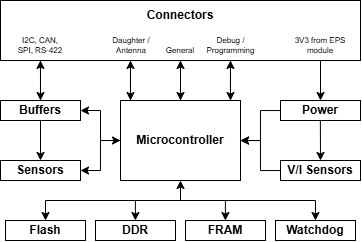
\includegraphics[scale=0.8]{images/arquitetura geral.png}
    \caption{Esquema geral de arquitetura.}
    \label{fig:arq_geral}
    \fonte{Elaboração própria.}
\end{figure}

Como podemos verificar, o microprocessador será crucial e deverá ter pinos suficientes para interface com todas as memórias, sensores e para se comunicar com os outros módulos do CubeSat. Além disso, a parte dedicada às tensões usadas deverá ser cuidadosamente feita, para suportar a potência dissipada por todos os componentes da placa de circuito impresso. A escolha de cada componente será descrita nas seções a seguir, respeitando sempre os seguintes critérios:

\begin{itemize}
	\item O componente deve funcionar corretamente nas temperaturas entre -40°C e 85°C;
	\item Circuitos integrados devem possuir herança de voo sempre que possível;
	\item Caso o circuito integrado necessite de um circuito específico, o mesmo deve conter itens preferencialmente dispostos na ECSS-Q-ST-60C, na NPSL ou similar aos mesmos, especialmente componentes discretos (capacitores, resistores, indutores, diodos, transistores, entre outros);
\end{itemize}

\subsection{Microcontrolador}

Como visto na Tabela \ref{tab:Tab_Missoes}, a fabricante com maior herança de voo estudada é a Xilinx, em especial os chips da família Zynq 7000, que são SoCs (\textit{System on a Chip}). Após um estudo próprio, o SoC Zynq 7030 se mostrou mais adequado pelas seguintes características:

\begin{itemize}
	\item Foi usado em missões extensivas em pequenos satélites (Gomspace, 2024), ou seja, possui herança de voo em missões similares em LEO e em CubeSats;
	\item Possui um envelopamento com 484 pinos, suficiente para prover as conexões necessárias para todas as interfaces requeridas (UG865, 2021);
	\item Capaz de rodar um sistema Linux (KADI et al.,2013);
	\item Por ser um SoC, possui alta adaptabilidade e flexibilidade, disponibilizando no mesmo chip uma FPGA (\textit{Field-Programmable Gate Array}) e um microprocessador, denominados respectivamente de PL e PS;
\end{itemize}

\subsection{Memórias}

As memórias serão necessárias para realizar operações, armazenar dados externos e internos e armazenar parâmetros de configuração do OBDH e de outros subsistemas do CubeSat. Para cada uma dessas funções uma memória diferente é necessária, seguindo suas características principais, sendo elas: tempo de acesso, tamanho do armazenamento e volatilidade.

\subsubsection{Memórias voláteis}

Partindo do princípio que a robustez e versatilidade estão alinhadas com a velocidade da memória, bem como sua capacidade de armazenamento máximo, a principal opção se tornou as memórias do tipo DDR (\textit{Double Data Rate}), que utilizam ambas a borda de subida e de descida para transferência de dados, atingindo o dobro de largura de banda de uma memória com SDR (\textit{Single Data Rate}) para uma mesma frequência de relógio (JEDEC, 2008). Essa relação pode ser ilustrada pela Figura \ref{fig:sdrvsddr}, onde pode-se verificar a transferência de dados do sinal DQ em relação ao sinal de relógio (bCLK e CLK) para SDR e DDR.

\begin{figure}[H]
    \centering
    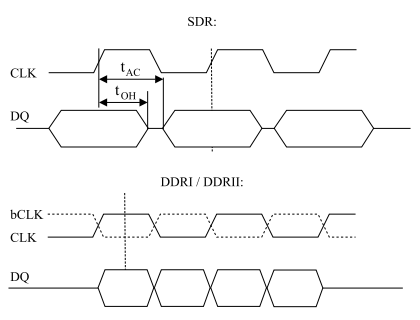
\includegraphics[scale=1]{images/ddrsdr.png}
    \caption{Comparação entre DDR e SDR.}
    \label{fig:sdrvsddr}
    \fonte{KLEHN E BROX, 2003.}
\end{figure}
 
Por essa razão, foi escolhida uma memória do tipo DDR3, com capacidade de 2Gb e frequência de operação de 800 MHz.

\subsubsection{Memórias não voláteis}

No caso das memórias não voláteis, é necessária uma atenção especial ao tipo de dado que será armazenado em cada uma delas. Para o caso de dados críticos, é preciso de uma memória que possua alta resistência aos efeitos da radiação, mantendo-se um compromisso com os tempos de escrita e leitura. Por sua vez, para dados de inicialização são mais críticos os tempos de leitura, enquanto para uma memória de dados mais gerais, o importante é o armazenamento total. Por meio desses critérios, foi possível avaliar, por meio da Tabela \ref{tab:memnvol}, o tipo de memória ideal para cada caso.

\begin{table}[H]
	\ABNTEXfontereduzida
	\caption{\label{tab:memnvol}Tabela comparativa de memórias não voláteis.}
	%\begin{tabular}{@{}p{2cm}p{2cm}p{2cm}p{2cm}p{2cm}p{2cm}p{3cm}@{}}
    \centering
    \begin{tabular}{@{} >{\centering}p{2cm} >{\centering}p{3cm} >{\centering}p{3cm} >{\centering}p{3cm}>{\centering}p{3cm} @{}}
    
		\toprule
		\textbf{Memória} & \textbf{Tempo de leitura} & \textbf{Tempo de escrita} & \textbf{Tolerância à radiação} & \textbf{Armazenamento máximo} \tabularnewline 
        \midrule
        Flash NOR & Rápido & Lento & Ruim & Regular\tabularnewline
        
        \midrule
        Flash NAND & Rápido & Lento & Ruim & Bom \tabularnewline 

        \midrule
        FRAM & Rápido & Rápido & Bom & Ruim \tabularnewline 
        
        \bottomrule
	\end{tabular}
	\fonte{Adaptado de GERARDIN E PACCAGNELLA, 2010.}
\end{table}

Com isso, foi então escolhida uma FRAM (\textit{Ferroelectric Random-Access Memory}) para armazenar dados críticos, uma Flash NAND para armazenamento de dados gerais e uma Flash NOR para armazenar o boot do sistema Linux no SoC.

\subsection{Conversores DC-DC}
Nos sistemas CubeSat do SpaceLab da UFSC, o módulo responsável pelo fornecimento de potência é o chamado EPS (MARCELINO, 2024). A partir disso, partindo do pressuposto que haverá uma tensão fornecida de 3,3 V, pode-se inferir a cascata de potência a partir do mesmo. Para o caso do Zynq e da memória DDR3, circuitos integrados são necessários para gerar as seguintes tensões: 

\begin{itemize}
	\item Zynq: 1 V e 1,8 V; 
	\item DDR3L: 1,35 V e 0,675 V.
\end{itemize}

Todos os demais periféricos devem aceitar uma tensão de alimentação de 3,3 V. Outro ponto importante são os circuitos de proteção contra \textit{latch-up}, um efeito similar a um curto-circuito na trilha de alimentação de circuitos CMOS (AN-600, 1989). 

\subsection{Sensores e Periféricos}
Como dito nos pré-requisitos, alguns sensores precisam estar presentes no OBDH. Entre eles:

\begin{itemize}
	\item Um monitor de tensão, para todas as tensões importantes do sistema;
	\item Um sensor de corrente para a tensão de entrada do módulo;
	\item Um giroscópio para medir a velocidade angular em órbita;
	\item Um magnetômetro para medição do campo magnético da Terra em órbita;
	\item Um WDT para reiniciar o sistema em caso de falha de software.
\end{itemize}

\section{Visualização da Arquitetura Proposta}

Depois das decisões tomadas, foi possível montar um diagrama, apresentado na Figura \ref{fig:arq}, que mostra cada circuito do computador de bordo. Aqui, por simplicidade, foram suprimidos os transceptores do protocolo CAN (\textit{Controller Area Network}) e a parte de potência do módulo. 

\begin{figure}[H]
    \centering
    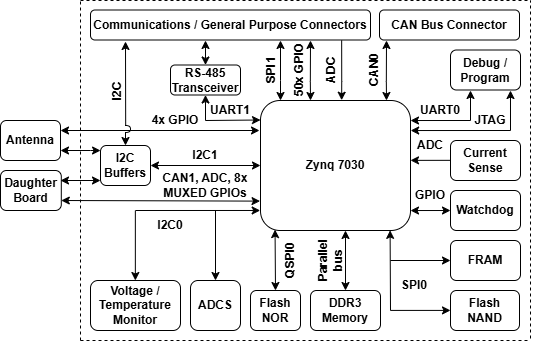
\includegraphics[scale=0.8]{images/arquitetura final.png}
    \caption{Arquitetura proposta para o OBDH.}
    \label{fig:arq}
    \fonte{Elaboração própria.}
\end{figure}

Também foram levadas em consideração as interfaces disponibilizadas pelo SoC, os componentes escolhidos e os conectores necessários. Os componentes escolhidos se encontram na Tabela \ref{tab:componentes}, conjuntamente com as interfaces requeridas para cada um, suas tensões de alimentação e suas correntes máximas no terminal de alimentação, no pior caso especificado pelo fabricante.

\begin{table}[H]
	\ABNTEXfontereduzida
	\caption{\label{tab:componentes}Informações sobre os componentes escolhidos.}
	%\begin{tabular}{@{}p{2cm}p{2cm}p{2cm}p{2cm}p{2cm}p{2cm}p{3cm}@{}}
    \centering
    \begin{tabular}{@{} >{\centering}p{2cm} >{\centering}p{4cm} >{\centering}p{2cm} >{\centering}p{3cm}>{\centering}p{3cm} @{}}
    
		\toprule
		\textbf{Componente} & \textbf{Número do Fabricante} & \textbf{Interface} & \textbf{Tensão de Alimentação} & \textbf{Corrente máxima} \tabularnewline 
        \midrule
        FRAM & CY15B104QN-50SXI & SPI & 3,3 V & 3,7 mA \tabularnewline
        
        \midrule
        Flash NOR & MT25QL128ABB1ESE-0AUT & QSPI & 3,3 V & 55 mA \tabularnewline 

        \midrule
        Flash NAND & MT29F1G01ABAFDSF-AAT:F & SPI & 3,3 V & 35 mA \tabularnewline 

        \midrule
        DDR3L & MT41K256M8DA-125:K & Paralela & 1,35 V & 182 mA \tabularnewline 

        \midrule
        WDT & TPS3823-33QDBVRQ1 & - & 3,3 V & 10 mA \tabularnewline 

        \midrule
        Monitor de Temperatura e Tensão & LTC2991IMS\#TRPBF & I2C & 3,3 V &  1,5 mA \tabularnewline 

        \midrule
        Sensor de Corrente & INA180A2IDBVR & - & 3,3 V & 1 mA \tabularnewline 

        \midrule
        Giroscópio & A3G4250D & I2C & 3,3 V & 7 mA \tabularnewline 

        \midrule
        Magnetômetro & MMC5983MA & I2C & 3,3 V & 0,45 mA \tabularnewline 

        \midrule
        Buffer I2C & TCA4311ADR & I2C & 3,3 V & 7 mA \tabularnewline 

        \midrule
        Transceptor CAN & A3G4250D & CAN & 3,3 V & 60 mA \tabularnewline 

        \midrule
        Transceptor RS-485 & THVD1451DR & Serial & 3,3 V & 3 mA \tabularnewline 

        \midrule
        Conversor DC-DC & TPS82085SILR & - & 3,3 V & - \tabularnewline 

        \midrule
        Conversor DC-DC para DDR3 & TPS51200DRCR & - & 3,3 V & 1 mA \tabularnewline 

        \midrule
        \textit{Load Switch} & TPS22920YZPR & - & 3,3 V & 0,2 mA \tabularnewline 
        
        \bottomrule
	\end{tabular}
	\fonte{Elaboração própria com base nos Datasheets de cada componente.}
\end{table}

\subsection{Estimativa de Potência Consumida}

A fim de garantir o funcionamento correto dos conversores DC-DC e seus respectivos periféricos, foi necessária uma estimativa da potência total consumida por todas as tensões disponíveis no módulo. Para isso, foi utilizada a Tabela \ref{tab:componentes}, bem como o datasheet de cada componente. No caso do SoC, sua fabricante disponibiliza uma planilha (XPE, 2019) para estimativas de potência em cada tensão de alimentação. 

Com isso, foram obtidos os valores da Tabela \ref{tab:estpow}, considerando uma eficiência de conversão de 85\% (TPS82085, 2019), já incluindo as estimativas de potência e os piores casos descritos anteriormente.

\begin{table}[H]
	\ABNTEXfontereduzida
	\caption{\label{tab:estpow}Estimativas de potência consumida.}
	%\begin{tabular}{@{}p{2cm}p{2cm}p{2cm}p{2cm}p{2cm}p{2cm}p{3cm}@{}}
    \centering
    \begin{tabular}{@{} >{\centering}p{2cm} >{\centering}p{4cm} >{\centering}p{4cm} >{\centering}p{4cm}@{}}
    
		\toprule
		\textbf{Tensão [V]} & \textbf{Potência Dissipada na Tensão [W]} & \textbf{Potência dissipada na tensão de 3,3 V [W]} & \textbf{Corrente máxima da trilha [A]} \tabularnewline 
        \midrule
         1,00 & 2,20 & 2,59 & 2,20 \tabularnewline
        
        \midrule
        1,35 & 0,25 & 0,29 & 0,18 \tabularnewline 

        \midrule
        1,80 & 0,63 & 0,74 & 0,35 \tabularnewline

        \midrule
        3,3 & 7,5 & - & 2,27  \tabularnewline        

        \bottomrule
	\end{tabular}
	\fonte{Elaboração própria.}
\end{table}

Através dessas estimativas, pode-se confirmar que o sistema de potência proposto suporta os componentes escolhidos e suas tensões e variações, mesmo quando se considera o pior caso.